\documentclass{report}
\usepackage[utf8]{inputenc}
\usepackage[spanish]{babel}
\usepackage{graphicx}
\usepackage{titlesec}
\usepackage{caption}
\usepackage{verbatim}

% Título, autores y fecha
\title{\Huge Predicción de comportamiento de clientes en canal web}
\author{Diego Oyarce Trejo \\ doyarce@utem.cl \and
        Marcelo Tapia Riquelme \\ marcelo.tapiar@utem.cl \and
        Cristobal González Gárate \\ cristobal.gonzalezg@utem.cl
        }
\date{\today}

\renewcommand{\contentsname}{Índice}

\begin{document}

\begin{titlepage}
  \centering  
  
\includegraphics[width=0.3\textwidth]{img/logoutem.png}  
  \vspace{1cm}
  
  \textsc{\LARGE Facultad de Ingeniería}  
  \vspace{0.5cm}
  
  \textsc{\LARGE Escuela de Informática}
  {\let\newpage\relax\maketitle}
\end{titlepage}

\tableofcontents

\listoffigures

\setcounter{section}{1}

\chapter{Presentación del proyecto}
\newpage

\section{Resumen}
El presente documento de Trabajo de Titulación resume exhaustivamente el proceso completo llevado a cabo para desarrollar un modelo de aprendizaje automático capaz de predecir el comportamiento de los usuarios en la nueva plataforma virtual de AFP Capital. Además de detallar la creación de este modelo, se enfoca en la relevancia de la predicción del comportamiento de los clientes y su valor estratégico para las empresas en la actualidad, destacando la importancia de obtener y manejar datos precisos sobre sus comportamientos.

El documento explora varios modelos de aprendizaje considerados como opciones viables, profundizando en la implementación detallada de tres modelos específicos y presentando los resultados obtenidos. Se destaca el proceso de selección del modelo más eficiente entre los evaluados, describiendo minuciosamente este modelo elegido y documentando las pruebas realizadas para demostrar su eficacia final.

Además del desarrollo del modelo, se aborda la creación de un servicio consumible que genera predicciones utilizando el modelo mencionado. Se describe la implementación de una API que facilita la generación de predicciones basadas en los datos de entrada necesarios para el modelo.

El proyecto concluye con la dockerización de todo el trabajo realizado, lo que permite su despliegue simplificado en la plataforma virtual de la empresa. Este enfoque busca garantizar la accesibilidad y la facilidad de implementación del servicio.

Finalmente, se incluyen recomendaciones para mejorar y continuar con el proyecto en caso de que la empresa desee seguir utilizando este modelo. Además, se presentan conclusiones y reflexiones del grupo de trabajo sobre el desarrollo y los hallazgos alcanzados durante el proyecto.

\textbf{Palabras clave:}  Afiliado, Administradora de Fondos de Pensiones, API (Application Programming Interfaces), EDA (Exploratory Data Analysis), Algoritmos de predicción, Algoritmos de clasificación, Modelos de predicción, ETL (Extract, Transform and Load), ARIMA (Modelo de Autorregresión integrada de media móvil), SARIMA (Modelo Estacional de Autorregresión integrada de media móvil), Redes Neuronales Artificiales (ANN), Redes LSTM (Long Short-Term Memory), Redes Neuronales Recurrentes (RNN).

\section{Palabras Clave}
\begin{singlespace}
    \begin{itemize}
        \item Afiliado
        \item Administradora de Fondos de Pensiones
        \item API (Application Programming Interfaces)
        \item EDA (Exploratory Data Analysis)
        \item Algoritmos de predicción
        \item Algoritmos de clasificación
        \item Modelos de predicción
        \item ETL (Extract, Transform and Load)
    \end{itemize}
\end{singlespace}

\section{Descripción del trabajo de título}
El trabajo de título se basa en un proyecto que requiere el procesamiento de la data de logs pasados de navegación del sitio web privado de AFP Capital, para detección de comportamientos de clientes y sus preferencias de uso, permitiendo navegaciones futuras customizadas. La lectura de logs será posible gracias a la extracción de dicha información desde Kibana (ElasticSearch), la cual es registrada por APIs variadas que se consumen en el sitio web. Elementos fundamentales del proyecto es el análisis exploratorio de datos, extracciones, transformaciones, cargas, modelo de predicción y detección de preferencias. 

\section{Objetivos}
\subsubsection{Objetivo general}
Analizar el comportamiento de los clientes y sus preferencias de uso en un período igual o inferior a 6 meses, para predecir navegaciones futuras personalizadas. 

\subsubsection{Objetivos específicos }
\begin{itemize}
    \item Realizar una investigación de las herramientas utilizadas para la predicción de comportamiento de usuarios en un canal web.
    \item Llevar a cabo un análisis y estudio de los datos entregados por la empresa. 
    \item Realizar un proceso ETL con la información de navegación web de los clientes de AFP Capital, para analizar su comportamiento dentro del sitio web privado. 
    \item Desarrollar un modelo capaz de predecir el comportamiento de los clientes de AFP Capital, para entregar navegaciones personalizadas futuras.
    \item Establecer recomendaciones de personalización en función de los hallazgos del modelo de predicción para futuras navegaciones dentro del sitio web de AFP Capital.
\end{itemize}

\section{Alcances y Limitaciones}
\subsubsection{Alcances}

El proyecto contempla los siguientes alcances:

\begin{itemize}
\item Se analizará el comportamiento de los clientes de AFP Capital en su nuevo sitio web privado.
\item El proyecto entregará un modelo capaz de predecir el comportamiento de los clientes de AFP Capital en el sitio web, así como una API que permita obtener recomendaciones de comportamiento personalizadas para un afiliado específico.
\end{itemize}

\subsubsection{Limitaciones}

El proyecto tiene las siguientes limitaciones:

\begin{itemize}
\item No se contará con acceso directo a las bases de datos de AFP Capital, por lo tanto, se trabajará con una muestra de datos.
\item No se podrá acceder a información sensible de los clientes de AFP Capital, como los RUTs (Rol Único Tributario) u otra información personal identificable.
\item El análisis se basará únicamente en datos cualitativos de la navegación web de los usuarios.
\end{itemize}

\chapter{La empresa}
\newpage

\section{Historia}
La historia de AFP Capital se remonta a noviembre de 1980, cuando se implementó en Chile el sistema de pensiones de capitalización individual. El 16 de enero de 1981, se constituyó la sociedad Administradora de Fondos de Pensiones Santa María, que más tarde se transformaría en AFP Capital S.A. Desde sus inicios, la empresa se destacó por su filosofía de servicio, enfocada en satisfacer las necesidades y expectativas de sus afiliados. 
En 1995, AFP Capital estableció la filial Santa María Internacional S.A., con el propósito de expandir su alcance y ofrecer servicios a personas naturales o jurídicas del extranjero, así como invertir en AFP o sociedades relacionadas con materias previsionales en otros países. Esta iniciativa consolidó la presencia de AFP Capital en el ámbito internacional y fortaleció su posición como una administradora de fondos de pensiones líder en la región. 
En el año 2000, se produjo una relevante transacción en la historia de AFP Capital. ING Group adquirió Aetna Inc., incluyendo el 96,56\% de las acciones de AFP Capital S.A. Esta adquisición tuvo como objetivo reforzar la posición de liderazgo de AFP Capital en el mercado previsional chileno y contribuir a su crecimiento y desarrollo. 
Posteriormente, en 2008, AFP Capital llevó a cabo una fusión con AFP Bansander, otra reconocida administradora de fondos de pensiones en Chile. Esta fusión permitió consolidar aún más las operaciones de AFP Capital y fortalecer su presencia en el país. A fines de 2011, Grupo SURA, una empresa líder en el negocio de pensiones en Latinoamérica, adquirió las operaciones de ING en la región. Esta adquisición llevó a AFP Capital a formar parte de Grupo SURA y a beneficiarse de su amplia experiencia y recursos, consolidándose como una compañía destacada en el mercado previsional latinoamericano. En resumen, la historia de AFP Capital está marcada por su constante evolución, consolidación y liderazgo en el mercado de administración de fondos de pensiones en Chile. A lo largo de los años, ha demostrado su compromiso con la excelencia en la prestación de servicios previsionales y su capacidad de adaptación a los cambios y desafíos del entorno económico y regulatorio.

\begin{figure}[H]
    \begin{minipage}[t]{0.9\textwidth}
        \caption{Historia AFP Capital}
        \label{historia-afp}        
    \end{minipage}

    \vspace{10pt}

    \begin{minipage}[b]{1.1\textwidth}
        \centering
        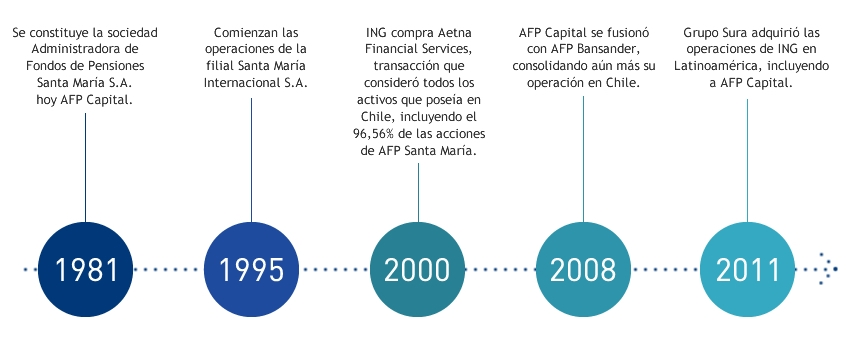
\includegraphics[width=\textwidth]{img/historia-afp-capital.jpg}        
    \end{minipage}

    \begin{minipage}[t]{0.9\textwidth}
        Fuente: AFP Capital. Recuperado de \url{https://www.afpcapital.cl/Quienes-Somos/Paginas/Historia.aspx}
    \end{minipage}
\end{figure}
%agregar la imágen de la historia%

\section{Descripción general}
\input{La empresa/Descripción general}

\section{Misión y visión}
\subsubsection{Misión}
La misión de AFP Capital es: "Acompañamos a nuestros clientes, a través de una asesoría experta y diferenciadora en soluciones de ahorro para alcanzar su número, su Pensión, creciendo sustentablemente, desarrollando a nuestros colaboradores e integrándose responsablemente a la comunidad." \cite{afpcapital} 

\subsubsection{Visión}
La visión de AFP Capital es: "Somos Guías, acompañamos a nuestros clientes a lograr sus sueños a través del ahorro." \cite{afpcapital}

\chapter{Marco teórico}
\newpage

\section{Definición e importancia de la predicción del comportamiento de un cliente dentro de un sitio web }
La predicción del comportamiento del cliente dentro de un entorno web se considera a la aplicación de técnicas y modelos analíticos para lograr predecir en cierta manera las posibles necesidades, acciones, preferencias y decisiones que un cliente pueda tomar mientras interactúa en alguna plataforma en línea o sitio web. En los últimos años, ha sido de gran importancia la predicción del comportamiento de los clientes para las empresas, gracias a esto buscan anticipar las necesidades y preferencias de sus clientes, pudiendo adaptar los productos y servicios para entregar una mayor satisfacción al cliente (Zheng, Thompson, Lam, Yoon y Gnanasambandam, 2013). La lealtad de los clientes representa un valor clave para las empresas, ya que un cliente leal seguirá consumiendo los productos y servicios de la empresa, por lo que si se mejora la experiencia del usuario, la satisfacción del cliente aumenta y esto genera un aumento en la ganancia de la empresa. 
Según Zheng, Thompson, Lam, Yoon y Gnanasambandam (2013), la predicción del comportamiento del cliente ayuda a las empresas a identificar oportunidades de mejora y mercado, además de ayudar a tomar decisiones informadas sobre estrategias de publicidad y marketing. El objetivo fundamental de predecir el comportamiento del cliente en un entorno web es lograr comprender y anticipar las acciones de los clientes con la meta de personalizar, mejorar la experiencia de usuario y poder aumentar la satisfacción y fidelidad de los clientes. 
Las predicciones pueden abarcar distintos aspectos del comportamiento de un cliente dentro de un canal web, a grandes rasgos existen 4 tipos de predicciones que se pueden realizar, están las predicciones de compras, donde mediante el análisis de patrones de navegación, su historial de compras, preferencias y características demográficas, gracias a esto se busca predecir las compras futuras de un cliente, se encuentra la predicción de clics, esta busca anticipar los enlaces o elementos con los cuales un cliente va a interactuar dentro de un sitio web, lo que busca mejorar la calidad de contenido que se encuentra desplegado y lograr mejorar la usabilidad del sitio web, también está presente la predicción de abandono de carrito, esta permite tomar acciones de recuperación o retención del cliente, se concentra en identificar aquellos clientes que agregan productos a un carrito de compra pero no finalizan el proceso de compra y por ultimo, esta la predicción de retención de clientes, esta busca predecir qué clientes están más cercanos a abandonar o terminar la relación existente con el sitio web, para poder generar e implementar estrategias para aumentar la fidelización y retención de estos clientes. 



\section{Comportamiento del Cliente/Afiliado en el canal web}

\subsection{Definición del comportamiento del cliente y su importancia para el negocio.}
Considerando los modelos de negocios establecidos por las Administradoras de Fondos de Pensiones [AFP], de ahí radica la importancia de la figura del cliente. Según lo que indica la Real Academia Española, el cliente es la persona que realiza una compra o utiliza los servicios que un profesional o empresa pueda ofrecer (Real Academia Española, s.f), no obstante en base al sistema establecido por las Administradoras de Fondos de Pensiones, el cliente obtiene el nombre de afiliado pues estos contribuyen o se encuentran inscritos en un plan de pensiones (Rasekhi, Fard y Kim, 2016). 
El afiliado es el centro del negocio, cuya gran importancia radica principalmente en la rentabilidad que brinda. Cada trabajador que decida afiliarse se traduce en una ganancia, mientras que cada afiliado que decida desafiliarse genera perdida. Considerando esto es que se puede apreciar la segunda importancia del afiliado, debido a que este promueve la marca si es que la experiencia del servicio de cara al usuario es buena. En tercer lugar, el afiliado, al ser un ganancia para el modelo, este a su vez que obtiene el servicio es capaz de posibilitar el crecimiento de la empresa al tener su preferencia. Por otro lado, la experiencia del cliente y su feedback es valiosa ya que puede brindar conocimiento de los puntos débiles y con posibilidad de mejora que tiene el sistema (Rodriguez, 2023). 
Dentro de las distintas funciones que el cliente tiene, en primer lugar se puede mencionar al cliente como consumidor. Consiste en unas de las funcionalidades más tradicionales puesto que el objetivo intrínseco del cliente es consumir o contratar servicios. Como consumidor es quien adquiere un producto o servicio y lo aprovecha para un fin o necesidad, por lo que la empresa obtiene su principal fuente de ingresos.
En segundo lugar, se tiene al cliente como prosumidor, en otras palabras, consume y produce a la vez (Toffler, 1980). Al momento del consumo, el cliente también deja reseñas o realiza comentarios en lugares especializados, información que resulta de utilidad para generar insights que mejoren la experiencia en el servicio. 
En tercer lugar, se entiende al cliente como crítico, puesto que si la experiencia del cliente es negativa, el feedback y reseñas negativas que este brinde pueden ser de índole constructiva como destructiva. 
En cuarto lugar, se encuentra el cliente como pieza fundamental en el desarrollo de los productos y servicios. Los comentarios de los clientes pueden conducir al desarrollo de servicios innovadores apegados a las necesidades que los clientes indican. Para poder lograr perfeccionar el servicio y productos ofrecidos, es crucial el aporte de los clientes recurrentes o suscriptores del servicio, en el caso específico de las Administradoras de Fondos de Pensiones se refiere a los afiliados. 
En quinto lugar, el cliente como evaluador de la experiencia. Relacionado con los puntos anteriores, la mejor forma de mejorar la experiencia del cliente es tomando en consideración los comentarios de los clientes en esta materia, así se puede generar una diferencia de las otras empresas que constituyen la competencia existente en el mercado. 
Por último, se considera que el cliente puede ser un eventual embajador de la marca, en otras palabras promotores de la misma pudiendo generar recomendaciones, comentarios y reseñas positivas que promuevan el negocio. 


\subsection{Características del comportamiento del cliente en el canal web.}
Para comprender la experiencia y el comportamiento del cliente en un canal web, es importante reconocer la existencia del customer journey, el cual describe las distintas etapas por las que un cliente pasa al consumir un producto o servicio. Según \cite{lemon2016customer}, estas etapas incluyen la conciencia, investigación, consideración, compra, uso y evaluación. La etapa de conciencia refiere a la identificación de una necesidad o problema que debe ser resuelto, mientras que la investigación implica la búsqueda de información por parte del cliente para encontrar posibles soluciones y comparar entre diferentes opciones disponibles. Luego, en la etapa de consideración, el cliente evalúa las alternativas y elige la que mejor se adapte a sus necesidades, lo que lleva a la etapa de compra, donde se realiza la contratación o adquisición del servicio seleccionado. Posteriormente, viene la etapa de uso, en la cual el cliente experimenta y evalúa la calidad, funcionalidad y experiencia del servicio. Por último, se encuentra la etapa de evaluación, en la cual el cliente emite un feedback voluntario, tanto positivo como negativo, sobre su experiencia satisfactoria o insatisfactoria. En resumen, las opciones disponibles en el canal web buscan hacer del customer journey una experiencia eficiente y agradable.

En cuanto al segundo párrafo, parece contener información específica sobre el canal web de AFP Capital y las opciones disponibles para los afiliados. Sin embargo, la estructura y organización del texto pueden mejorarse para una mayor claridad. Aquí está el párrafo revisado:

Para acceder al canal web de AFP Capital, es necesario ser afiliado y contar con una cuenta privada personal que incluya el RUT y contraseña. Una vez ingresado al canal web privado, los afiliados tienen a su disposición diversas opciones para satisfacer sus necesidades. Estas incluyen revisión del pago o no de la cotización mensual, la obtención de certificados de cotizaciones, afiliación, antecedentes previsionales y traspaso de fondos, así como certificados tributarios. Además, se pueden obtener certificados generales, como de residencia, suscripción de ahorro previsional voluntario (APV), cuenta 2, remuneraciones imponibles, periodos no cotizados y trabajo pesado. En el caso de afiliados pensionados, también se pueden obtener certificados de asignación familiar, calidad de pensionado, pensiones pagadas, pensión en trámite, ingreso base y comprobante de pago de pensión. Además, es posible acceder a la cartola en línea. El canal web privado permite realizar el ahorro obligatorio y voluntario, inversiones, depósitos directos, consultar planillas de pagos y ver las comisiones cobradas como afiliado. También ofrece la opción de verificar el fondo de pensiones, los tipos de fondos disponibles (A, B, C, D, E) y sus porcentajes de rentabilidad, así como realizar cambios de fondo de pensiones y acceder a educación previsional. Además, se brinda la posibilidad de realizar giros en cuentas personales, acceder a rescates financieros y tramitar la pensión.

\subsection{Factores que influyen en el comportamiento del cliente}
%Factores que influyen en el comportamiento del cliente en el canal web, tales como la usabilidad y el diseño del sitio web.
Lemon y Verhoef (2016) proponen que los principales factores que influyen en el comportamiento del usuario y su experiencia son sensoriales, afectivos, cognitivos, puntos de contacto y externos. Dentro de la experiencia sensorial se encuentra lo apreciable con alguno de los sentidos del cuerpo, tanto vista, olor, tacto, entre otros. Respecto de la experiencia afectiva, hay que tener en consideración la emocionalidad del cliente producto de la experiencia del producto o del servicio. Al hablar del aspecto cognitivo, este refiere de los pensamientos, creencias y/o actitudes que el cliente pueda tener respecto de la compañía, el producto o el servicio entregado. Sobre los puntos de contacto, estos hacen mención a las distintas maneras en las que el cliente y la compañía entran en contacto, tales como la publicidad, servicio al cliente, redes sociales o interacciones de tipo transaccional (Lemon y Verhoef, 2016). Por último, el factor externo cuya definición hace referencia a considerar el contexto actual, las condiciones socioeconómicas y otros factores que puedan afectar la experiencia del usuario que se encuentren fuera de control de la compañía. 
Dentro de los factores que pueden influir en el comportamiento de un cliente en el canal web están principalmente, la usabilidad y el diseño. Respecto a la usabilidad, esta depende de 7 características las que garantizan una buena experiencia del usuario. Según Sanchez (2011) la accesibilidad, legibilidad, navegabilidad, facilidad de aprendizaje, velocidad de utilización, eficiencia del usuario y tasas de error del canal web, influyen en la experiencia y posterior feedback que el usuario pueda brindar sobre el uso de los servicios. 
Por otro lado, el diseño del sitio web depende de 5 características para garantizar un buen contenido y estética para lograr que el usuario encuentre lo que busca en el menor tiempo posible, en otras palabras, eficiencia. El autor Walter Sanchez (2011) indica que el diseño debe de ser entendible, novedoso, comprensible, inteligente y atractivo, consiguiendo acercar los contenidos de mejor manera al usuario y logrando conseguir una navegación más intuitiva. Estos factores son de gran importancia para que el usuario pueda encontrar el contenido que busca en el menor tiempo posible y que la experiencia sea positiva al interactuar con la interfaz del sitio web. 


\section{Herramientas para la predicción del comportamiento del cliente en el canal web}

\subsection{Introducción a las herramientas de análisis de datos y su aplicación en el contexto del comportamiento del cliente}
En el entorno empresarial actual, la capacidad de tomar decisiones informadas y basadas en datos se ha vuelto fundamental para el éxito y la competitividad de las organizaciones. El análisis de datos desempeña un papel crucial en este proceso, permitiendo a las empresas obtener información valiosa a partir de grandes volúmenes de datos y utilizarla para comprender el comportamiento del cliente de manera más profunda y precisa. Esto resulta de suma importancia, ya que la calidad de las decisiones tomadas marca la diferencia entre el éxito y el fracaso \cite{analitica-predictiva}.

Dentro de las herramientas de análisis de datos, se destacan cuatro conceptos clave que han revolucionado la forma en que se procesan y se obtiene información de los datos: Business Intelligence, Big Data, Machine Learning y Data Mining. Estas herramientas proporcionan a las empresas la capacidad de extraer conocimientos y patrones significativos de los datos, lo que a su vez les permite tomar decisiones estratégicas más acertadas y personalizar sus estrategias de marketing y atención al cliente.

El Business Intelligence (BI) se refiere a la recopilación, análisis y presentación de datos empresariales para facilitar la toma de decisiones. Mediante el uso de diversas técnicas y herramientas, el BI permite a las empresas visualizar y comprender mejor los datos de sus operaciones y clientes. Esto incluye la generación de informes, el análisis de tendencias, la monitorización de indicadores clave de rendimiento (KPI) y la creación de tableros de control interactivos. El BI ayuda a las organizaciones a identificar oportunidades, detectar áreas de mejora y optimizar su rendimiento en función de datos históricos y en tiempo real. Sobre la inteligencia de negocios, se ha determinado que cada implementación es única para cada proceso empresarial \cite{analitica-empresarial}.

El Big Data se refiere a la gestión y análisis de grandes volúmenes de datos, tanto estructurados como no estructurados, que superan la capacidad de las herramientas tradicionales de almacenamiento y procesamiento. El Big Data se caracteriza por las tres V's: Volumen (gran cantidad de datos), Velocidad (alta velocidad de generación y procesamiento de datos) y Variedad (diversidad de fuentes y formatos de datos). Para aprovechar el potencial del Big Data, las empresas emplean técnicas de procesamiento distribuido y herramientas específicas para el almacenamiento, procesamiento y análisis de estos datos masivos. El análisis de Big Data permite identificar patrones, tendencias y correlaciones ocultas en los datos, lo que brinda información valiosa para entender y anticipar el comportamiento del cliente.

El Machine Learning (aprendizaje automático) es una rama de la inteligencia artificial que permite a los sistemas informáticos aprender y mejorar automáticamente a partir de la experiencia sin ser programados explícitamente. En lugar de basarse en una analítica descriptiva, el Machine Learning ofrece una analítica predictiva \cite{inteligencia-negocios}. Mediante algoritmos y modelos, el Machine Learning permite a las empresas analizar grandes conjuntos de datos y detectar patrones complejos en el comportamiento del cliente. Esto permite realizar predicciones y recomendaciones personalizadas, así como automatizar tareas y procesos, lo que mejora la eficiencia operativa y la experiencia del cliente.

El Data Mining (minería de datos) se refiere al proceso de descubrir información valiosa, patrones y relaciones desconocidas en grandes conjuntos de datos. Utilizando técnicas estadísticas y algoritmos avanzados, el Data Mining permite identificar correlaciones y tendencias ocultas en los datos, lo que ayuda a las empresas a comprender mejor el comportamiento del cliente y tomar decisiones más acertadas. Esta herramienta es especialmente útil para la segmentación de clientes, la detección de fraudes, la recomendación de productos y la personalización de ofertas.


\subsection{Métodos, técnicas y tecnologías de análisis de datos utilizados en la predicción del comportamiento del cliente}
En el análisis de datos para predecir el comportamiento del cliente, se utilizan una variedad de métodos, técnicas y tecnologías que permiten procesar y analizar grandes volúmenes de información con el fin de obtener información valiosa. Estas herramientas proporcionan a las empresas y organizaciones la capacidad de comprender mejor a sus clientes, identificar patrones y tendencias, y tomar decisiones estratégicas más acertadas.

Entre los métodos y modelos más utilizados se encuentran la regresión logística, que permite predecir la probabilidad de que un cliente realice una determinada acción o tome una decisión; el clustering, que agrupa a los clientes en segmentos o categorías similares con características y comportamientos comunes; los árboles de decisión, que representan un conjunto de reglas lógicas para clasificar a los clientes en diferentes grupos; el Random Forest, que combina múltiples árboles de decisión para mejorar la precisión de las predicciones; y el Gradient Boosting Machine, que utiliza múltiples modelos de aprendizaje débiles para construir un modelo más robusto y preciso.

Además de los métodos y modelos, existen diversas técnicas que se aplican en el análisis de datos para predecir el comportamiento del cliente. Entre ellas se encuentran las redes neuronales artificiales (ANN), que son modelos inspirados en el funcionamiento del cerebro humano y se utilizan para reconocer patrones y realizar predicciones complejas; y el Support Vector Machine (SVM), que es un algoritmo de aprendizaje automático utilizado para clasificar y predecir datos.

En cuanto a las tecnologías utilizadas en el análisis de datos, se destacan diversas herramientas y lenguajes de programación. Algunas de las más populares son Tableau, que permite visualizar y explorar los datos de manera interactiva; Python, con bibliotecas como Pandas, NumPy y Scikit-learn, que ofrecen una amplia gama de funciones y algoritmos para el análisis de datos; R, con paquetes como dplyr, caret y randomForest, que brindan herramientas estadísticas y de aprendizaje automático; Apache Spark, que permite procesar y analizar grandes volúmenes de datos de manera distribuida; KNIME y RapidMiner, que son plataformas de análisis de datos visuales; y QlikView y Power BI, que son herramientas de visualización de datos y creación de tableros de control.

\subsection{Modelos de predicción del comportamiento del cliente}
%Modelos de predicción del comportamiento del cliente en el canal web
Existen diferentes modelos empleados para realizar predicciones del comportamiento de un usuario en un canal web, el empleo de dichos modelos se encuentran explicados a continuación:

\subsubsection{Modelos de regresión}
El modelo de regresión es empleado para la predicción de variables, la regresión logística estima la probabilidad de que suceda un evento basándose en un conjunto de datos. Existen 3 tipos de modelos de regresión, los cuales corresponden a los modelos de regresión logística binaria, regresión logística multinomial y regresión logística ordinal.

Siendo el Modelo de regresión lógica binaria es empleado para predecir comportamientos de variables que tienen un comportamiento dicotómico, es decir, que solo cuentan con dos resultados posibles, como ejemplo podemos mencionar a la clasificación de correo electrónico si es spam o no lo es, si una opción es verdadero o falso, entre otros ejemplos. Dentro de la regresión logística es el más utilizado y en general, corresponde a uno de los clasificadores más comunes para la clasificación binaria.

El Modelo de regresión logística multinomial es empleado para predecir cuando la variable dependiente cuenta con tres o más resultados posibles, cabe recalcar que los valores a predecir no se encuentran ordenados.

Finalmente, el Modelo de regresión logística ordinal es utilizado cuando la variable de respuesta tiene tres o más resultados posibles, pero a diferencia del modelo de regresión logística multinomial, los valores empleados si poseen un orden definido.

\subsubsection{Ventajas de los modelos de regresión}

\begin{itemize}
    \item La implementación del modelo es más sencillo comparado con otros modelos.
    \item Interpretación de los resultados relativamente sencilla.
    \item Simplificación de problemas.
    \item Existencia de documentación respecto a los modelos.
\end{itemize}

\subsubsection{Desventajas de los modelos de regresión}

\begin{itemize}
    \item Propensos a sobreentrenarse.
    \item Alta sensibilidad a valores atípicos.
    \item Son propensos a realizar suposiciones.
\end{itemize}

\subsubsection{Modelos de recomendación}
Los modelos de recomendación corresponden a una subclase de aprendizaje automático que es utilizado para clasificar o valorar productos y usuarios. En modo de resumen, es un sistema de recomendación en un sistema que predice las valoraciones que un usuario puede dar a un producto y/o servicio. Este modelo es empleado en grandes empresas como Google, Amazon, Instagram, Spotify, entre otros.

Este modelo se puede clasificar en sistemas de filtrado colaborativo, sistemas basados en contenido o sistema de recomendación híbrido.

Los sistemas de filtrado colaborativo corresponden al proceso en el cual se predicen los intereses de un usuario, esto se realiza al identificar las preferencias e información de varios usuarios, realizando una búsqueda de patrones utilizando de filtrado de información.

Los sistemas basados en contenido se enfocan en generar recomendaciones basadas en las preferencias y los perfiles de usuario. El modelo trata de hacer coincidir a los usuarios con elementos o productos que les hayan gustado anteriormente. Un punto a destacar de este sistema es que se basa en los productos destacados por el usuario objetivo, en cambio, los otros modelos se basan en el usuario y en otros usuarios que utilizan la plataforma.

Para terminar con los modelos de recomendación, los sistemas de recomendación híbridos se encuentran diseñados para utilizar diferentes fuentes de información para generar las recomendaciones. 

\subsubsection{Ventajas de los modelos de recomendación}
\begin{itemize}
    \item Aumenta la participación de los usuarios.
    \item Recomendación de elementos acorde a los gustos de los usuarios.
    \item Poseen la capacidad de automatizar sus sugerencias.
\end{itemize}

\subsubsection{Desventajas de los modelos de recomendación}
\begin{itemize}
    \item Propenso a presentar sesgo y falta de diversificación.
    \item Autorización de terceros por privacidad (dado que utilizan datos personales).
    \item Presentan problemas de arranque en frío.
    \item Difíciles de interpretar.
\end{itemize}

\subsubsection{Modelos de series temporales}
 
Los modelos de series temporales corresponden a un proceso en el cual son utilizados datos pasados con la finalidad de predecir acontecimientos futuros. Estos modelos analizan tendencias y patrones en los datos para extraer información para realizar predicciones sobre valores futuros, este tipo de modelos son utilizados en el ámbito financiero para predecir ventas o cotizaciones, otro de los campos en los que es empleado este modelo es en el científico, enfocándose en predecir los patrones meteorológicos. 

\subsubsection{Ventajas de los modelos de series temporales}
\begin{itemize}
    \item Capaces de capturar patrones.
    \item Útiles para predecir a corto plazo.
    \item Proporcionan facilidades para la interpretación de los resultados.
\end{itemize}

\subsubsection{Desventajas de los modelos de series temporales}
\begin{itemize}
    \item No son eficientes para predecir a largo plazo.
    \item Son muy sensibles a los datos atípicos.
    \item Requieren información consistente.
\end{itemize}

\subsubsection{Modelos de aprendizaje automático}
Los modelos de aprendizaje automático corresponden a programas capaces de identificar patrones o tomar decisiones. Estos pueden ser entrenados para realizar predicciones, identificar objetos e imágenes, también puede ser empleado para predecir comportamientos de usuarios.

\subsubsection{Ventajas de los modelos de aprendizaje automático}
\begin{itemize}
    \item Permiten trabajar con grandes volúmenes de datos.
    \item Permite la automatización de tareas.
    \item Mejoran a medida que son utilizados.
\end{itemize}

\subsubsection{Desventajas de los modelos de aprendizaje automático}
\begin{itemize}
    \item Vulnerables a ataques de terceros.
    \item Requieren de una capacidad significativa de recursos.
    \item Algunos modelos entregan resultados complicados de interpretar.
\end{itemize}

\subsubsection{Modelos de análisis de sentimientos}
Como dice el nombre, el modelo de análisis de sentimientos permite procesar y analizar información a tiempo real, es utilizado principalmente en las redes sociales para analizar cómo ve la gente un producto nuevo y lo que no les gusta a sus clientes.

\subsubsection{Ventajas de los modelos de análisis de sentimientos}
\begin{itemize}
    \item El modelo es escalable.
    \item Permite la automatización de los procesos del modelo.
    \item Permite segmentar y personalizar los métodos de análisis.
\end{itemize}

\subsubsection{Desventajas de los modelos de análisis de sentimientos}
\begin{itemize}
    \item Al modelo se le dificulta identificar el sarcasmo.
    \item Posee limitaciones al momento de identificar sentimientos complejos.
    \item Los resultados del modelo pueden verse afectados por sesgos en los datos de entrenamiento.
\end{itemize}

\subsubsection{Modelos de detección de anomalías}
Los modelos de detección de anomalías corresponden a modelos de machine learning enfocados en detectar actividades extrañas en la información que está analizando, con esto queremos decir que detecta anomalías.

Existen diferentes tipos de métodos para detectar anomalías con machine learning, entre ellos se encuentran los modelos supervisados, sin supervisión y semi supervisado.

Para el método de modelos supervisados, el entrenamiento del modelo consta de dos variables de entrenamiento: normal y anormal. El modelo utiliza los ejemplos para detectar patrones y detectar anomalías en los datos proporcionados. Es importante destacar que, en el entrenamiento supervisado es fundamental asegurar la calidad de los datos con el cual será entrenado el modelo.

Para el método de modelos sin supervisión, es común emplear redes neuronales para implementar el modelo, dado que al utilizar redes neuronales se disminuye la carga de trabajo manual, con esto queremos decir que no es necesario preparar los datos de antemano. Un punto negativo es que la dificultad de implementar una red neuronal es alta.

Finalmente, para el modelo semi supervisado es una combinación de los dos métodos anteriores, permitiendo contar con las ventajas de ambos métodos. Al ser supervisado durante su entrenamiento, es posible tener un mayor control del tipo de patrones que aprender el modelo.

\subsubsection{Ventajas de los modelos de detección de anomalías}
\begin{itemize}
    \item El modelo permite automatizar la detección de anomalías.
    \item Posee gran adaptabilidad a datos y entornos.
    \item Permite detectar de manera temprana las anomalías.
\end{itemize}

\subsubsection{Desventajas de los modelos de detección de anomalías}
\begin{itemize}
    \item Es difícil definir una anomalía.
    \item Requiere de un entrenamiento adecuado al modelo.
    \item Es muy propenso a entregar posibles falsos positivos y falsos negativos.
\end{itemize}

\subsubsection{Modelos de atribución}
Los modelos de atribución permiten predecir el recorrido que los clientes seguirán al momento de concretar una compra. Este recorrido puede contener las redes sociales, el uso del sitio web del vendedor, el correo electrónico, entre otros. Los modelos de atribución permiten determinar el impacto que tiene el uso de las acciones para el sistema de marketing. 

Existen varios modelos adicionales para el uso del marketing y la predicción de comportamiento, sin embargo, para este proyecto se limitó la búsqueda a los modelos mencionados anteriormente, los cuales se adaptan mejor a nuestras necesidades.

\subsubsection{Ventajas de los modelos de atribución}
\begin{itemize}
    \item Facilita el rastrear de mejor manera el paso a paso del cliente.
    \item Permiten mayor personalización de rastreo de los clientes.
\end{itemize}

\subsubsection{Desventajas de los modelos de atribución}
\begin{itemize}
    \item Poseen una mayor complejidad que los otros modelos.
    \item La interpretación de los resultados puede ser subjetiva.
    \item Poseen limitaciones en la medición del seguimiento.
\end{itemize}


\subsection{Metodología del proyecto}
Para llevar a cabo el desarrollo del proyecto, se definieron cuatro fases que corresponden a la totalidad del proyecto, las cuales corresponden a:

\subsubsection{Fase 1: Planteamiento y planificación}

Para la primera fase del proyecto, se llevará a cabo una planificación de la manera en la que será abordada la problemática, para desarrollar un anteproyecto que será utilizado para evaluar y planificar las actividades correspondientes al desarrollo del proyecto. Entre ellas se encuentran:

\begin{itemize}
    \item Planteamiento del proyecto y sus objetivos.
    \item Definición de alcances y limitaciones.
    \item Creación de un cronograma de actividades.
\end{itemize}

\subsubsection{Fase 2: Investigación}

Para la segunda fase, se realizará una investigación de herramientas y recursos necesarios para llevar a cabo un diseño de la solución para la problemática del proyecto planteado, sumado a un análisis de las bases de datos brindadas por la empresa AFP Capital. Una vez realizado lo anterior, se llevará a cabo una propuesta de diseño para la problemática, siendo entregada y analizada por la empresa, con la finalidad de pasar a desarrollo. Algunas de las actividades de esta fase corresponden a:

\begin{itemize}
    \item Investigación del problema.
    \item Toma de requerimientos.
    \item Investigación de tecnologías de análisis de datos.
\end{itemize}

\subsubsection{Fase 3: Modelamiento y desarrollo}
Para la tercera fase, se llevará a cabo el diseño y desarrollo del sistema propuesto, además de realizar pruebas para verificar el correcto funcionamiento. Algunas de las actividades de esta fase corresponden a:

\begin{itemize}
    \item Modelado del sistema ETL.
    \item Modelado de la API.
    \item Implementación del modelo propuesto.
    \item Pruebas y validaciones.
    \item Correcciones de errores.
\end{itemize}

\subsubsection{Fase 4: Conclusiones y recomendaciones}
Para la última fase, se dará fin al desarrollo del proyecto, elaborando un manual de usuario el cual indicaría algunas funcionalidades del sistema. Algunas de las actividades de esta fase corresponden a:

\begin{itemize}
    \item Desarrollo de manual de usuario.
    \item Redacción de conclusiones y recomendaciones.
    \item Cierre del proyecto.
\end{itemize}


\subsection{Metodología del Sistema}
\subsubsection{CRISP-DM}
La metodología CRISP-DM (Cross-Industry Standard Process for Data Mining) es un proceso estándar utilizado para realizar proyectos de minería de datos. La metodología CRISP-DM se divide en seis fases distintas que se describen a continuación:

\begin{enumerate}
    \item \textbf{Comprensión del problema:} En esta fase se define el problema a resolver y se establecen los objetivos del proyecto. También se recopilan los datos necesarios para el proyecto.
    \item \textbf{Comprensión de los datos:} En esta fase se realiza una exploración de los datos para comprender su calidad, estructura y relevancia para el problema en cuestión.
    \item \textbf{Preparación de los datos:} En esta fase se limpian y procesan los datos para que puedan ser utilizados en la etapa de modelado.
    \item \textbf{Modelado:} En esta fase se aplican técnicas de modelado para desarrollar un modelo predictivo. Se prueban diferentes modelos y se selecciona el que mejor se ajuste a los datos.
    \item \textbf{Evaluación:} En esta fase se evalúa el modelo desarrollado en la fase anterior. Se verifica que el modelo funcione correctamente y se ajuste adecuadamente a los datos.
    \item \textbf{Implementación:} En esta fase se implementa el modelo desarrollado en la fase de modelado en un entorno de producción. También se establecen planes para monitorear el rendimiento del modelo y actualizarlo según sea necesario.
\end{enumerate}

Las fases de la metodología CRISP-DM son iterativas, lo que significa que es posible volver a una fase anterior si es necesario.

\subsubsection{OSEMN}

La metodología OSEMN (acrónimo de las palabras en inglés: Obtain, Scrub, Explore, Model, Interpret) es un proceso utilizado en la minería de datos y el análisis de datos para trabajar con grandes conjuntos de datos de manera efectiva. 

\begin{enumerate}
    \item \textbf{Obtener (Obtain):} En esta etapa, se recopilan los datos necesarios para el análisis. Los datos pueden provenir de diferentes fuentes, como bases de datos, archivos en línea o registros de sensores. La calidad y la cantidad de los datos obtenidos son cruciales para el éxito del análisis.
    \item \textbf{Limpieza (Scrub):} Una vez que se han obtenido los datos, es necesario realizar una limpieza para eliminar datos innecesarios o incorrectos. Esta etapa puede implicar la eliminación de duplicados, la corrección de errores y la eliminación de valores atípicos. El objetivo de esta etapa es obtener datos limpios y coherentes para el análisis.
    \item \textbf{Exploración (Explore):} En esta etapa, se utilizan técnicas de visualización y estadísticas para explorar los datos y obtener información sobre ellos. Se pueden identificar patrones, tendencias y relaciones entre diferentes variables. El objetivo es obtener una comprensión más profunda de los datos y de cómo se relacionan entre sí.
    \item \textbf{Modelado (Model):} En esta etapa, se utilizan técnicas de modelado estadístico o de aprendizaje automático para crear modelos que puedan predecir resultados futuros o identificar patrones en los datos. El objetivo es utilizar los datos para crear un modelo que pueda utilizarse para tomar decisiones informadas.
    \item \textbf{Interpretación (Interpret):} En esta etapa, se interpretan los resultados obtenidos en la etapa de modelado. Los resultados pueden ser utilizados para tomar decisiones o para generar nuevas hipótesis que puedan ser exploradas en futuros análisis.
\end{enumerate}

Se propone el uso de la metodología OSEMN, ya que se enfoca en el análisis de datos y la creación de modelos predictivos. OSEMN también es una metodología más flexible que CRISP-DM, lo que puede ser útil en un proyecto de SCRUM donde se busca una mayor adaptabilidad.

Por otro lado, también se propone el uso de la metodología CRISP-DM, ya que el proyecto incluye una etapa de exploración y análisis de datos, seguida por una fase de construcción de modelos. CRISP-DM se enfoca en el proceso completo de minería de datos, desde la comprensión del problema hasta la implementación del modelo, lo que puede servir para realizar un trabajo más estructurado.

Ya que este proyecto se encuentra bajo el marco de trabajo SCRUM, ambas metodologías pueden ser utilizadas de manera complementaria, utilizando OSEMN para las fases de creación de modelos y CRISP-DM para la etapa de exploración y análisis de datos.


\chapter{Proceso ETL}
\newpage

\end{document}